\section{项目数据描述}

\begin{figure}[ht]
 \centering
 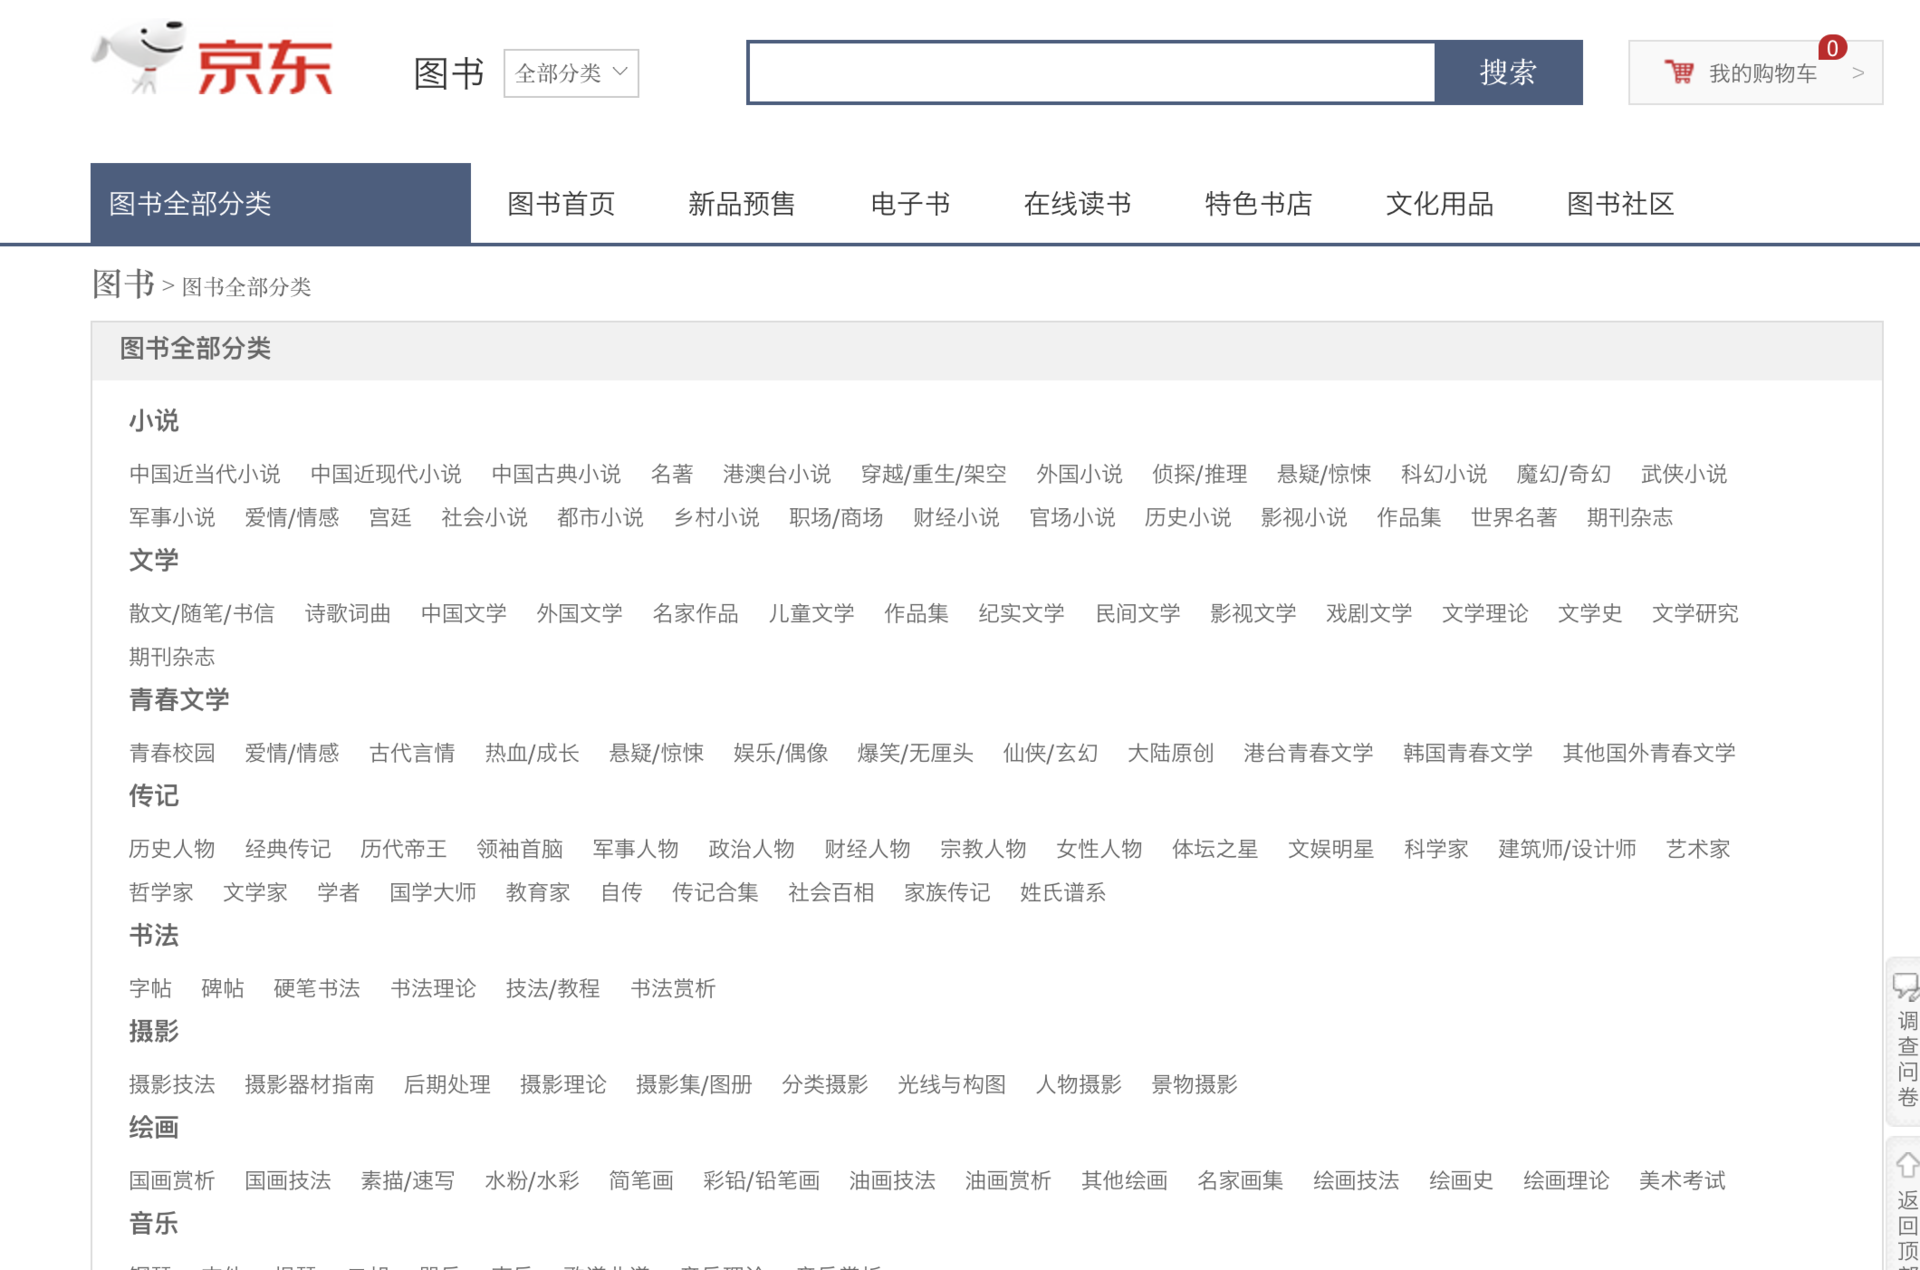
\includegraphics[height=8cm]{images/jd_book.jpg}
 \caption{京东图书类别\footnote{https://book.jd.com/booksort.html}}
 \label{fig:jd_book}
\end{figure}

\begin{figure}[ht]
 \centering
 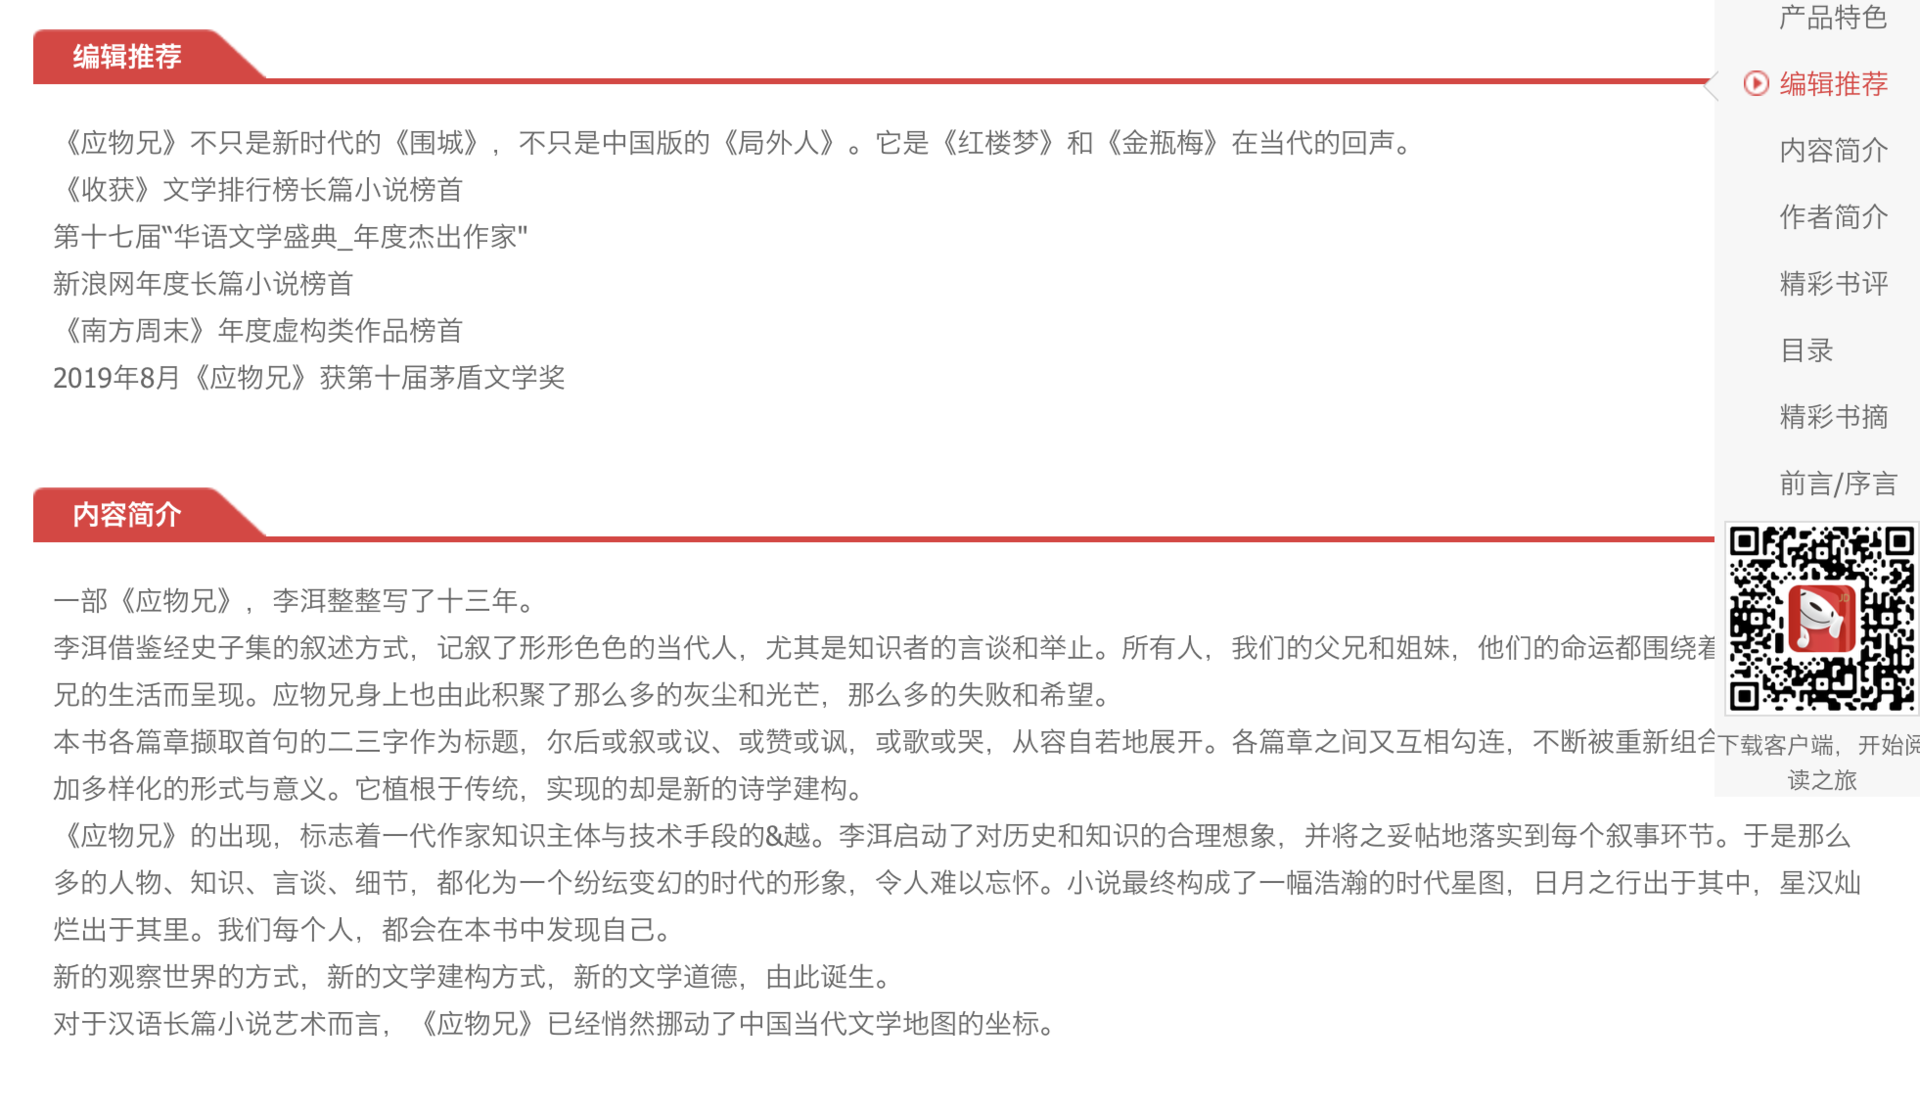
\includegraphics[height=7cm]{images/jd_book_text.jpg}
 \caption{京东图书内容简介}
 \label{fig:jd_book_text}
\end{figure}

\begin{figure}[ht]
 \centering
 
\includegraphics[height=4cm]{images/jd_book_cover.jpg}
 \caption{京东图书封面实例}
 \label{fig:jd_book_cover}
\end{figure}

\noindent 在本项目中,我们使用的是京东图书数据。在京东网站上,每一本图书都录属于列表中的一个类目,如图~\ref{fig:jd_book}所示。由于本项目中需要实现的是单标签多类别的分类模型,我们决定使用\textbf{图书的二级类目}作为样本的真实标签,比如“中国文学”,“纪实文学”,“青春校园”等。在给定的数据集中,一共包含$33$个不同类别的标签。\\

\noindent 对于标签的识别,我们使用两种类型的数据,分别为图书的文本内容简介(如图~\ref{fig:jd_book_text}所示)以及图书的封面图(如图~\ref{fig:jd_book_cover}所示)。\\

\nooindent 本项目使用的数据集中,一共包括206316个训练样本,58948个验证样本,29474个测试样本。